%!TEX root = ../report.tex
\section{Trainingssteuerung}
Trainingssteuerung ist die gewichtete kurz-, mittel- und langfristige Abstimmung und Ausführung aller Planungs-, Trainings-, Kontroll-, Auswertungs- und Lenkungsmaßnahmen eines Trainingsprozesses zur Erreichung der Trainingsziele.
\begin{figure}[H]
  \centering
  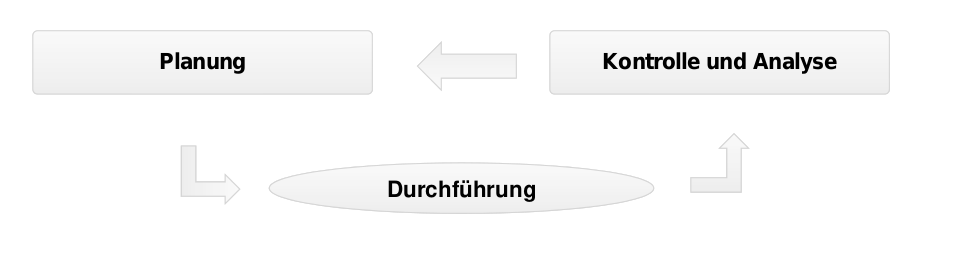
\includegraphics[width=.7\textwidth]{pictures/trainingssteuerung_komponenten.png}
\end{figure}

\subsection{Planung}
\begin{figure}[H]
  \centering
  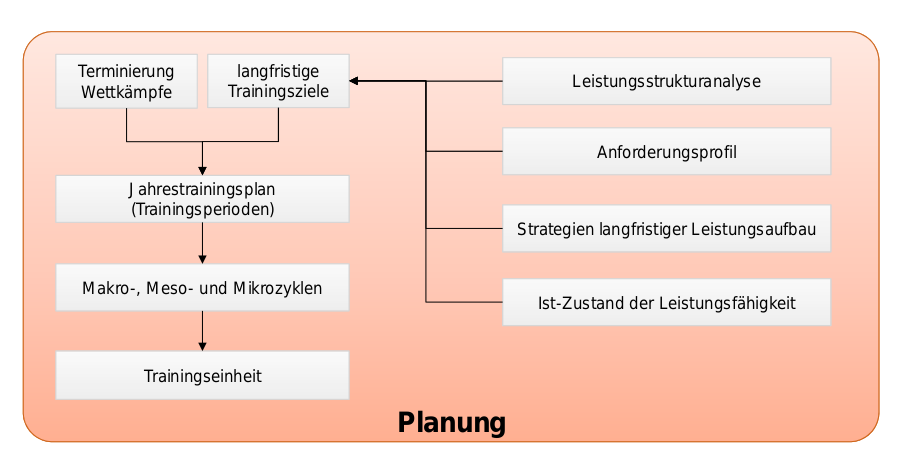
\includegraphics[width=.7\textwidth]{pictures/trainingsplanung_komponenten.png}
\end{figure}
\paragraph{Leistungsstrukturanalyse} Analyse aus welchen Komponenten die Leistung einer Sportart besteht.
Davon werden diejenigen ausgewählt, die besonders entscheidend für den Erfolg sind und werden maximiert.
Die übrigen nur optimiert.\\
\paragraph{Anforderungsprofil} beschreibt wie gut Fähigkeiten auf dem angestrebten Niveau ausgeprägt sein müssen.
Beinhaltet sind:
\begin{itemize}
  \item Leistungsnorm: ist die resultierende Wettkampfleistungen/Teilleistungen
  \item Konditionelle Norm
  \item technisch-taktische Norm
\end{itemize}
\paragraph{Langfristige Traingingsziele} werden mithilfe der Leistungsstrukturanalyse, dem Anforderungsprofil, der Wettkampfanalyse \& der Trainerphilosophie gesetzt.
Folgende fragen sind wichtig:
\begin{itemize}
  \item Ist die Trainierbarkeit gegeben? (Reaktionsschnelligkeit, Kraft)
  \item Lohnt sich das Training? (Abwägung von Niveau, Potential und Zeitbuget)
  \item Ist eine Integration in das Training möglich? (Konkurrenz der verschiedenen Komponenten im Zeitbuget, Wechselwirkungen der Komponenten)
\end{itemize}
\textbf{Planung einer Trainingseinheit}\\
\begin{figure}[H]
  \centering
  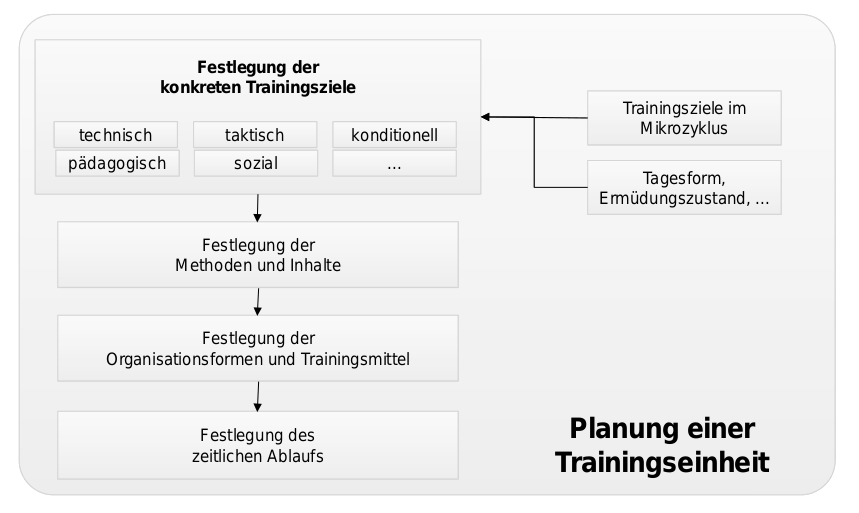
\includegraphics[width=.7\textwidth]{pictures/trainingssteuerung_planung_trainingseinheit.png}
\end{figure}
\begin{figure}[H]
  \centering
  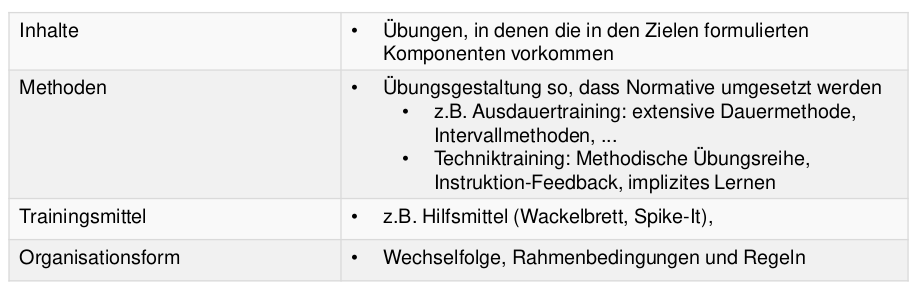
\includegraphics[width=.7\textwidth]{pictures/trainingssteuerung_planung_trainingseinheiten_komponenten.png}
\end{figure}
Zieldefinition:\\
\begin{figure}[H]
  \centering
  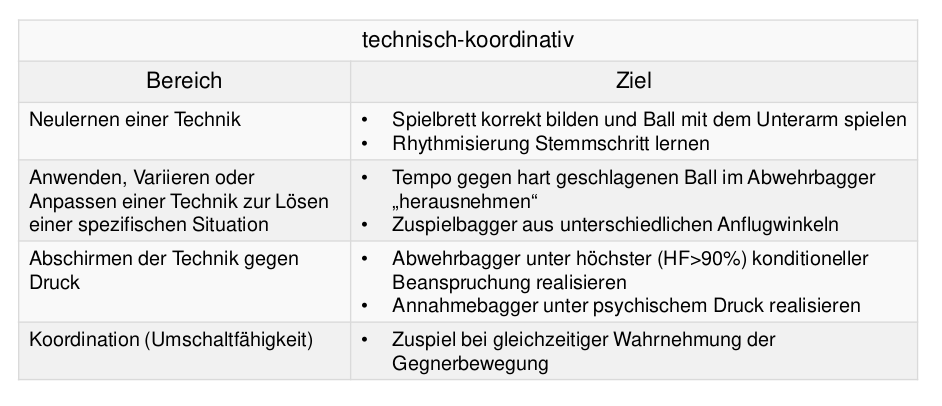
\includegraphics[width=.7\textwidth]{pictures/trainingssteuerung_zieldefinition_koordinativ.png}
\end{figure}
\begin{figure}[H]
  \centering
  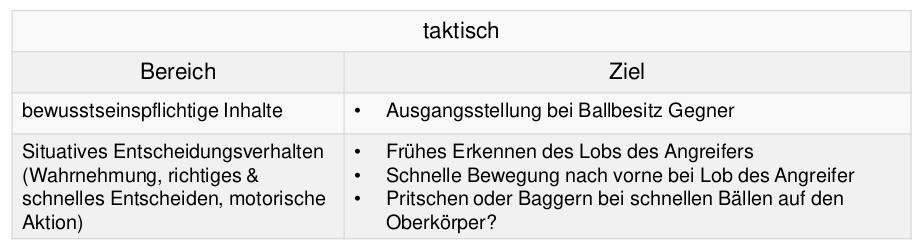
\includegraphics[width=.7\textwidth]{pictures/trainingssteuerung_zieldefinition_taktisch.png}
\end{figure}
\begin{figure}[H]
  \centering
  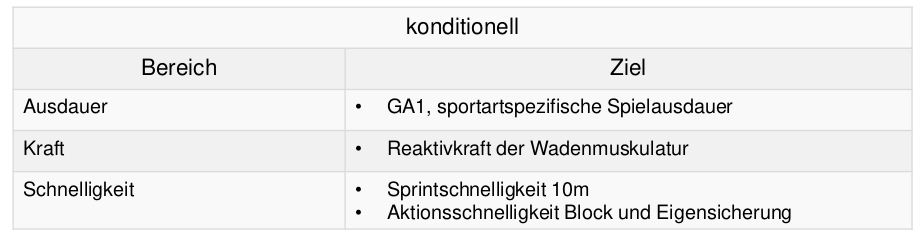
\includegraphics[width=.7\textwidth]{pictures/trainingssteuerung_zieldefinition_konditionell.png}
\end{figure}
Zeitlicher Ablauf einer Trainingseinheit:\\
Der Ablauf ist üblicherweise in drei Teile eingeteilt: Ein einleitender Teil, in dem eine mentale und physische Vorbereitung erfolgt, ein Hauptteil, in dem die Trainingsziele umgesetzt werden sollen und den Ausklang, in dem die Regeneration eingeleitet wird.\\
Im Hauptteil werden zunächst die Trainingsziele umgesetzt, die eher einen erholten Zustand erfordern, wie Schnelligkeit, Koordination oder Reaktion.
Gegen ende des Trainings werden dann vermehrt die anstrengenderen Trainingsziele in betracht gezogen, wie aerobe Ausdauer, Kraftausdauer oder Techniktrainingsabschrimung.

\subsection{Durchführung}
Kritisch überprüfen, ob Training wie geplant abläuft!
\begin{itemize}
  \item Technisch-Taktisch
    \begin{itemize}
      \item Entstehen die benötigten Situationen ausreichend häufig?
      \item Können Techniken in der Situation sinnvoll angewendet werden?
      \item Sind Entscheidungen richtig?
      \item Ist Feedback vorhanden?
    \end{itemize}
  \item Konditionell
    \begin{itemize}
      \item Werden die Normative erreicht (Belastung zu hoch, zu niedrig)? evtl.
      \item Pulskontrolle
      \item Sind Pausen zu lang, zu kurz?
      \item Intensitätssteuerung schwierig -> "mündiger Athlet" (Lenk)
    \end{itemize}
  \item Durchführung ggf.\ verändern (z.B.\ Organisationsform)
\end{itemize}

\subsection{Kontrolle und Analyse}
Es gibt drei verschiedene Arten von Diagnositken:
\begin{itemize}
  \item Leistungsdiagnostik ist die Beschreibung und Beurteilung der Leistung, der Teilleistungen und Leistungskomponenten. Erfasst werden Wettkampf(teil-)leistungen oft über spezielle motorische Tests.
  \item Wettkampfdiagnostik ist Leistungsdiagnostik im Wettkampf oder unter Wettkampfbedingungen
  \item Trainingsdiagnostik ist die Beschreibung und Beurteilung des Trainingsprozesses und seiner Wirkung (nicht Leistungsdiagnostik im Training).
    Dabei werden Trainingskomponenten wie Belastungen und Beanspruchungen erfasst.
    Komponenten:\\
    \begin{figure}[H]
      \centering
      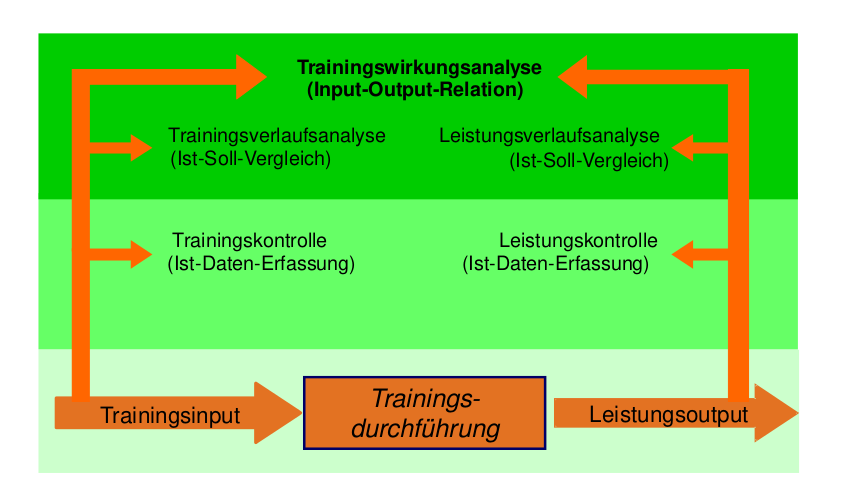
\includegraphics[width=.7\textwidth]{pictures/trainingssteuerung_trainingsdiagnostik_komponenten.png}
    \end{figure}
\end{itemize}

\subsection{Fitness-Fatigue-Modell}
Das Fitness-Fatigue-Modell beschreibt die Prognose und Leistungsentwicklung im Bezug auf die Trainingsbelastung.
Es besteht aus zwei antagonistischen Effekten des Trainings.
Die \textbf{Fitness} sind die resultierenden leistungssteigernden Effekte aus dem Training, die durch Anpassungen des Körpers hervorgerufen werden.
Die Ermüdung (\textbf{Fatigue}) repräsentiert die temporäre Ermüdung nach dem Training.
Aus diesen beiden Faktoren ergibt sich der aktuelle individuelle Leistungszustand.
\begin{figure}[H]
  \centering
  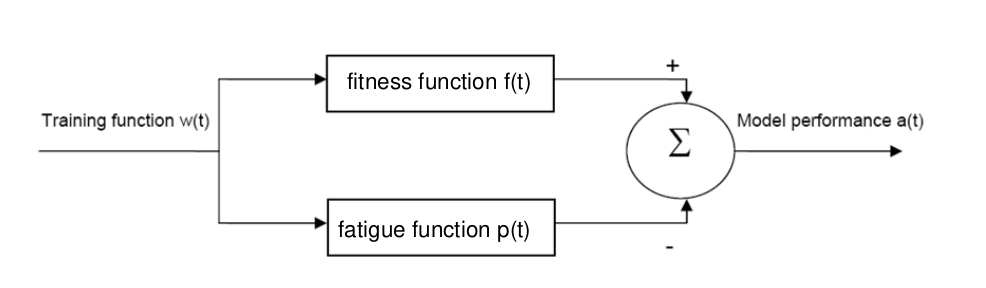
\includegraphics[width=.7\textwidth]{pictures/trainingssteuerung_ffm_trainingsfunction.png}
\end{figure}
\begin{description}
  \item[w(t)] beschreibt den Trainingsreiz zum Zeitpunkt t\\
    TRIMP (Trainings Impuls) = Umfang (Dauer, Anzahl,\ldots) $\cdot$ Intensität (Herzfrequenz, Laktat, V02,\ldots)\\
    Beispiel: 6km $\cdot$ 70\% = 420 TRIMS
  \item[f(t)] beschreiben den leistungssteigernden Effekt des Reizes zum Zeitpunkt t\\
    $\Delta f_i(t)=k_1 \cdot w_i \cdot e^{\frac{-(t-t_i)}{T1}}$ für $t\geq t_i$, $\Delta f_i(t)=0$ else\\
    $k_1$ = wie hoch ist der leistungssteigernde Effekt\\
    T1 = wie lange hält der leistungssteigernde Effekt an
  \item[p(t)] beschreiben den Ermüdungseffekt des Reizes zum Zeitpunkt t\\
    $\Delta p_i(t)=k_2 \cdot w_i \cdot e^{\frac{-(t-t_i)}{T2}}$ für $t\geq t_i$, $\Delta p_i(t)=0$ else\\
    $k_2$ = wie hoch ist der Ermüdungseffekt\\
    T2 = wie lange hält der Ermüdungseffekt an
  \item[a(t)] beschreibt den Leistungszustand zum Zeitpunkt t\\
    $\Delta a_i(t)=\Delta f_i(t) - \Delta p_i(t)$
\end{description}
T1, T2, $k_1$ und $k_2$ können individuell angepasst werden.
\begin{figure}[H]
  \centering
  \begin{subfigure}{.45\textwidth}
    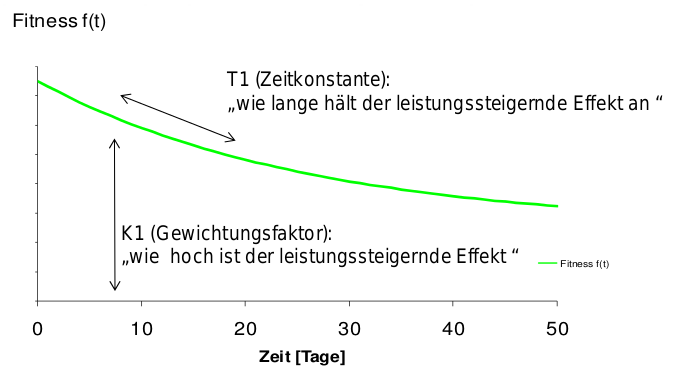
\includegraphics[width=\textwidth]{pictures/trainingssteuerung_fitnessfunktion.png}
    \caption{Fitnessfunktion}
  \end{subfigure}
  \begin{subfigure}{.45\textwidth}
    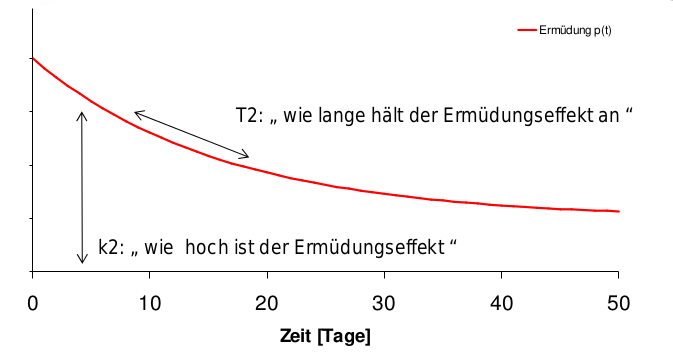
\includegraphics[width=\textwidth]{pictures/trainingssteuerung_fatiguefunktion.png}
    \caption{Fatiguefunktion}
  \end{subfigure}
  \begin{subfigure}{\textwidth}
    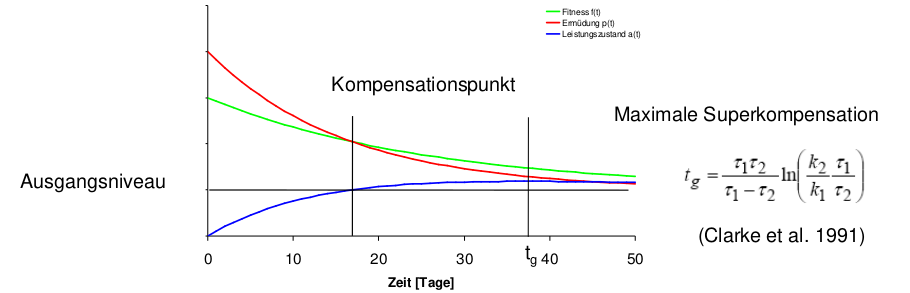
\includegraphics[width=\textwidth]{pictures/trainingssteuerung_leistungsfunktion.png}
    \caption{Leistungsfunktion}
  \end{subfigure}
\end{figure}
\textbf{Vorteile}
  \begin{itemize}
    \item Simulation auf Basis des
    \item Superkompensationsmodells möglich
  \end{itemize}
\textbf{Nachteile}
  \begin{itemize}
    \item Indexbildung über mehrere, unterschiedliche Reize
    \item Keine Erfassung unterschiedlicher Verzögerungen
    \item Keine Erfassung der Wechselwirkung
    \item Präzision der Zeitangaben?
    \item Im Wesentlichen für mks-Sportarten
  \end{itemize}

\subsection{Kybernetik vs.\ Synergetik}
\textbf{Kybernetik:} Der Organismus wird als einfache Maschine gesehen.
Der Trainingsprozess wird mithilfe eines Regelkreises beschrieben. 
Die Trainingsbelastung kann die Leistungsfähigkeit exakt steuern.
Hat sich nicht als effektiv bewiesen.\\
\textbf{Synergetik:} Der Organismus wird als dynamisches System gesehen, das aus rückgekoppelten oszilierenden Prozessen besteht.
Belastungen werden nicht „genau“ dosiert, sondern sie müssen sich lediglich im richtigen Bereich befinden, um Selbstorganisationprozesse auszulösen.

\subsection{Zusammenfassung}
\begin{itemize}
  \item Planung und Dokumentation!
  \item Klarheit über Ziele verschaffen
  \item Optimierung durch individuelle Trainingswirkungsanalysen
  \item Mathematische Modelle können helfen
  \item kritische Reflektion der Grundannahmen des kybernetischen Modells
\end{itemize}
